
\documentclass[tikz,border=0.5in]{standalone}

\usepackage{xcolor}
\usepackage{tikz}
\usetikzlibrary{arrows.meta,decorations.pathreplacing}

\pagestyle{empty}

\definecolor{strategyarrowone}{HTML}{A98EDA}
\definecolor{strategyarrowtwo}{HTML}{E58C9A}
\definecolor{strategyarrowthree}{HTML}{D1A647}

\definecolor{strategyarrowone}{HTML}{657BBB}
\definecolor{strategyarrowtwo}{HTML}{657BBB}
\definecolor{strategyarrowthree}{HTML}{657BBB}


\definecolor{parentlink}{HTML}{B7B2C2}
\definecolor{strategyink}{HTML}{657BBB}
\definecolor{strategyfill}{HTML}{F1F3FB}

\definecolor{figureink}{HTML}{253049}
\definecolor{codegreen}{HTML}{309F86}
\definecolor{codefill}{HTML}{EEF8F4}
\definecolor{uctborder}{HTML}{C45100}
\definecolor{uctfill}{HTML}{FFF0E3}
\definecolor{uctarrow}{HTML}{E06B1A}
\definecolor{ucttext}{HTML}{8C3500}
\definecolor{banditink}{HTML}{996B38}
\definecolor{banditfill}{HTML}{FFF7E8}

\begin{document}




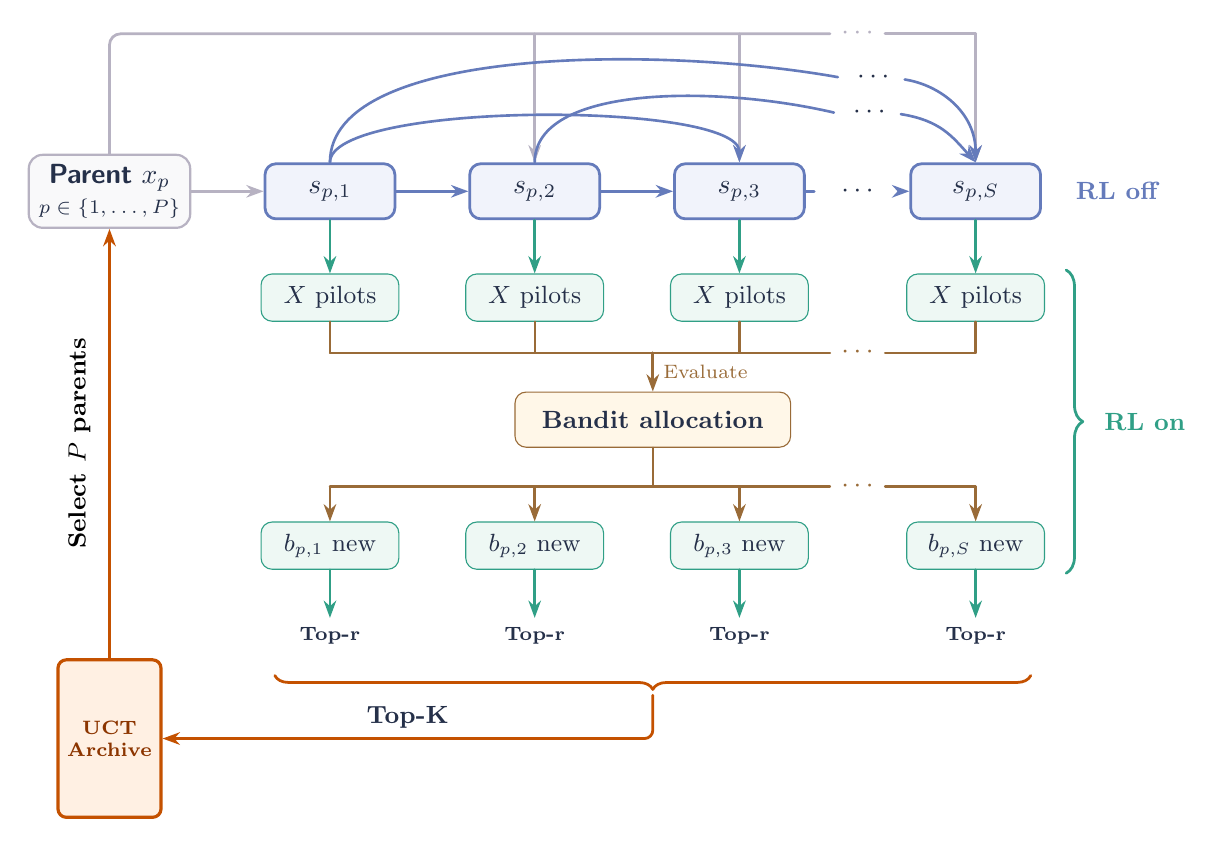
\begin{tikzpicture}[
  font=\sffamily,
  text=figureink,
  line cap=round,
  line join=round,
  arr/.style={
    -{Stealth[length=2.2mm,width=1.6mm]},
    line width=0.95pt
  },
  strategy/.style={
    rectangle,
    rounded corners=4pt,
    draw=strategyink,
    fill=strategyfill,
    line width=1pt,
    minimum width=1.65cm,
    minimum height=0.70cm,
    align=center
  },
  parent/.style={
    rectangle,
    rounded corners=5pt,
    draw=parentlink,
    fill=parentlink!8,
    line width=0.8pt,
    minimum width=2.05cm,
    minimum height=0.90cm,
    align=center
  },
  code/.style={
    circle,
    draw=codegreen,
    fill=codefill,
    line width=0.95pt,
    minimum size=0.50cm,
    inner sep=0pt,
    font=\scriptsize
  }
]



\node[parent] (parentnode) at (0,0)
  {\textbf{Parent} $x_p$\\[-1pt]
   {\scriptsize $p\in\{1,\ldots,P\}$}};

\node[strategy] (s1) at (2.8,0) {$s_{p,1}$};
\node[strategy] (s2) at (5.4,0) {$s_{p,2}$};
\node[strategy] (s3) at (8.0,0) {$s_{p,3}$};
\node[strategy] (sS) at (11.0,0) {$s_{p,S}$};

\draw[arr,draw=parentlink]
  (parentnode.east) -- (s1.west);

\draw[
  draw=parentlink,
  line width=1.0pt,
  rounded corners=4pt
]
  (parentnode.north)
  -- (0,2)
  -- (9.15,2);

\node[text=parentlink,inner sep=0pt] at (9.50,2) {$\cdots$};
\draw[draw=parentlink,line width=1.0pt]
  (9.85,2) -- (11.0,2);

\draw[arr,draw=parentlink]
  (5.4,2) -- (s2.north);

\draw[arr,draw=parentlink]
  (8.0,2) -- (s3.north);



\draw[arr,draw=parentlink]
  (11.0,2) -- (sS.north);

\draw[arr,draw=strategyarrowone]
  (s1.east) -- (s2.west);

\draw[arr,draw=strategyarrowtwo]
  (s2.east) -- (s3.west);

\draw[
  draw=strategyarrowthree,
  line width=0.95pt
]
  (s3.east) -- (8.95,0);

\node[
  fill=white,
  inner sep=1pt
]
  at (9.50,0)
  {$\cdots$};

\draw[arr,draw=strategyarrowthree]
  (10.05,0) -- (sS.west);

\draw[arr,draw=strategyarrowone]
  (s1.north)
  .. controls (2.8,1.15) and (8.0,1.15) ..
  (s3.north);

\draw[
  draw=strategyarrowone,
  line width=0.95pt
]
  (s1.north)
  .. controls (2.8,1.85) and (7.0,1.85) ..
  (9.25,1.45);

\node[
  fill=white,
  inner sep=1pt
]
  at (9.70,1.45)
  {$\cdots$};

\draw[arr,draw=strategyarrowone]
  (10.10,1.42)
  .. controls (10.55,1.35) and (11.0,1.00) ..
  (sS.north);

\draw[
  draw=strategyarrowtwo,
  line width=0.95pt
]
  (s2.north)
  .. controls (5.4,1.35) and (7.7,1.35) ..
  (9.20,1.00);

\node[
  fill=white,
  inner sep=1pt
]
  at (9.65,1.00)
  {$\cdots$};

\draw[arr,draw=strategyarrowtwo]
  (10.05,0.98)
  .. controls (10.55,0.90) and (10.70,0.70) ..
  (sS.north);

% ------------------------------------------------------------
% Pilot programs: generated and evaluated for every strategy
% ------------------------------------------------------------

\foreach \s/\x/\j in {s1/2.8/1,s2/5.4/2,s3/8.0/3,sS/11.0/S}{
  \node[
    draw=codegreen,fill=codefill,rounded corners=4pt,
    minimum width=1.75cm,minimum height=0.60cm,
    align=center,font=\small
  ] (pilot\j) at (\x,-1.35)
    {$X$ pilots};
  \draw[arr,draw=codegreen] (\s.south) -- (pilot\j.north);
}

% All pilot rewards feed one allocation decision for this parent.
\foreach \x/\j in {2.8/1,5.4/2,8.0/3,11.0/S}{
  \draw[draw=banditink,line width=0.85pt]
    (pilot\j.south) -- (\x,-2.05);
}
\draw[draw=banditink,line width=0.85pt]
  (2.8,-2.05) -- (9.15,-2.05);
\node[text=banditink,inner sep=0pt] at (9.50,-2.05) {$\cdots$};
\draw[draw=banditink,line width=0.85pt]
  (9.85,-2.05) -- (11.0,-2.05);

\node[
  draw=banditink,fill=banditfill,rounded corners=4pt,
  minimum width=3.50cm,minimum height=0.70cm,
  align=center,font=\small
] (bandit) at (6.9,-2.90)
  {\textbf{Bandit allocation}};

\draw[arr,draw=banditink]
  (6.9,-2.05) -- node[right,font=\scriptsize,text=banditink]
    {Evaluate} (bandit.north);

% Counts are allocated together; phase-2 generation remains parallel.
\draw[draw=banditink,line width=0.85pt]
  (bandit.south) -- (6.9,-3.75);
\draw[draw=banditink,line width=0.85pt]
  (2.8,-3.75) -- (9.15,-3.75);
\node[text=banditink,inner sep=0pt] at (9.50,-3.75) {$\cdots$};
\draw[draw=banditink,line width=0.85pt]
  (9.85,-3.75) -- (11.0,-3.75);

\foreach \x/\j in {2.8/1,5.4/2,8.0/3,11.0/S}{
  \node[
    draw=codegreen,fill=codefill,rounded corners=4pt,
    minimum width=1.75cm,minimum height=0.60cm,
    align=center,font=\small
  ] (phase\j) at (\x,-4.50)
    {$b_{p,\j}$ new};
  \draw[arr,draw=banditink]
    (\x,-3.75) -- (phase\j.north);

  \node[align=center,font=\scriptsize] (top\j) at (\x,-5.65)
    {\textbf{Top-r}};
  \draw[arr,draw=codegreen] (phase\j.south) -- (top\j.north);
}


% ------------------------------------------------------------
% Merge selected programs into the archive
% ------------------------------------------------------------

\draw[
  decorate,
  decoration={brace,mirror,amplitude=5pt},
  draw=uctborder,
  line width=1pt
]
  (2.10,-6.15) -- (11.70,-6.15);

\node[
  rectangle,
  rounded corners=3pt,
  draw=uctborder,
  fill=uctfill,
  text=ucttext,
  line width=1.15pt,
  minimum width=1.20cm,
  minimum height=2.00cm,
  align=center,
  font=\scriptsize\bfseries
] (uctarchive) at (0,-6.95)
  {UCT\\Archive};

\draw[arr,draw=uctborder,line width=1pt,rounded corners=3pt]
  (6.90,-6.40) -- (6.90,-6.95)
  -- node[midway,above,font=\small,text=figureink]
    {\textbf{Top-K}}
  (uctarchive.east);

\draw[arr,draw=uctborder,line width=1.15pt]
  (uctarchive.north)
  -- node[midway,rotate=90,above=3pt,
          font=\small\bfseries,text=black]
    {Select $P$ parents}
  (parentnode.south);

% ------------------------------------------------------------
% Labels
% ------------------------------------------------------------

\node[anchor=west,font=\small,text=strategyink]
  at (12.15,0) {\textbf{RL off}};
\draw[
  decorate,
  decoration={brace,amplitude=6pt},
  draw=codegreen,
  line width=1pt
]
  (12.15,-1.00) -- (12.15,-4.85)
  node[midway,right=10pt,font=\small,text=codegreen]
    {\textbf{RL on}};
\end{tikzpicture}

\end{document}
